\documentclass[a4paper,12pt]{article}
%For images
\usepackage{graphicx}
 
\addtolength{\oddsidemargin}{-.875in}
\addtolength{\evensidemargin}{-.875in}
\addtolength{\textwidth}{1.75in}
 
\addtolength{\topmargin}{-.875in}
\addtolength{\textheight}{1.75in}
 
\begin{document}
\begin{enumerate}
    \item 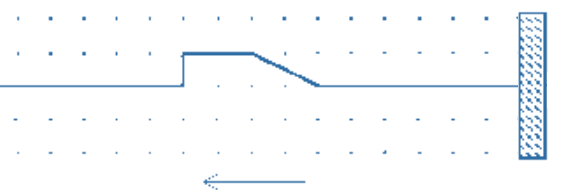
\includegraphics{Figur 1.png}
    
    \item 
    I det slutna röret så kommer sju noder att skapas,
    vilket är toppar och dalar vilket bildar följande bild:
    \begin{center}
        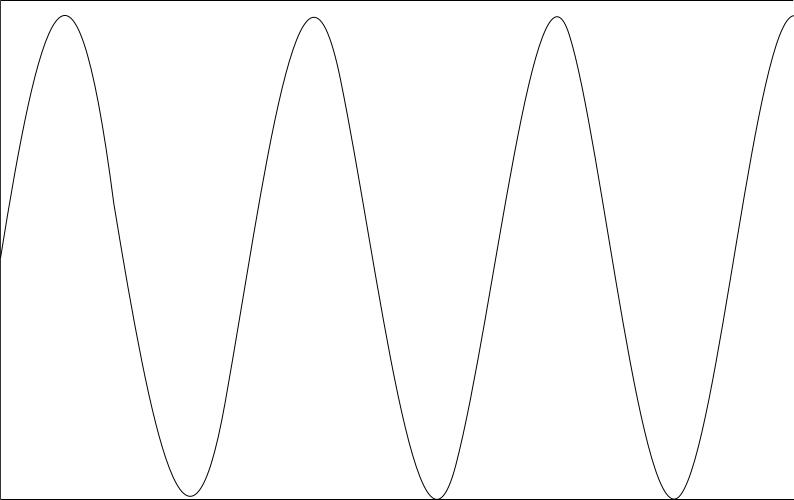
\includegraphics[scale=0.5]{Figur 2.png}
    \end{center}

    Vi kan observera att antalet våglängder som passerar
    är 13/4. Då får vi från ekvationerna att längden L är 
    likamed 13/4 gånger våglängden $\lambda$.

    $$L=\frac{13}{4}\lambda \Rightarrow \lambda=L\frac{4}{13}$$

    Med hastighetsekvationen blir det 

    $$v=f\lambda=fL\frac{4}{13}=870\cdot 1.5\cdot \frac{4}{13}\approx 402m/s$$

    \item 
\end{enumerate}
\end{document}